\documentclass[../Main.tex]{subfiles}

\begin{document}

\section{Entwicklung} \label{sec:Entwicklung}

\subsection{Levelgestaltung} \label{sec:Levelgestaltung}

\subsubsection{Gestaltung des Kampfabschnitts}

\begin{itemize}[leftmargin=1.5cm]
    \item \textcolor{red}{[Platzhalter] Konkrete Gestaltung des Kampfabschnitts aus den Designzielen: Raumlayout, Gegnerpositionen und Spawnpunkte, Wellenabfolge sowie Höhen- und Raumvariation.}
    \item \textcolor{red}{Direkteste Grundlagen laut Wissenslandkarte: Kapitel 1 (Encounter-Design), Kapitel 3 (Raumtypen) und Kapitel 4 (Pacing).}
    \item \textcolor{red}{Planung vor der Greybox gegebenenfalls mit einem Molekül- oder Bubble-Diagramm.}
\end{itemize}

\subsubsection{Umsetzung im Prototyp}

\begin{itemize}[leftmargin=1.5cm]
    \item \textcolor{red}{[Platzhalter] Umsetzung der Gestaltung in Godot: Greybox, Szenenaufbau und Gegnerplatzierung im Level.}
    \item \textcolor{red}{Architekturbezug laut Wissenslandkarte: Kapitel 2 (Kernmechanik) und Kapitel 10 (Modularität) begründen die Godot-Entscheidungen.}
    \item \textcolor{red}{Technische Details siehe Kapitel 5.}
\end{itemize}

\subsection{Technische Entwicklung}
\textcolor{red}{Rückmeldung irgendwas von 2 oder 3 weiteren dingern un zhile meinte noch 2 weitere dinger wären möglich}

\subsubsection{Gemeinsame Komponenten}

\paragraph{FloatingBody: Ein Algorithmus für sanfte Bewegung auf rauen Oberflächen}

Unser Ziel weshalb wir den \texttt{FloatingBody}-Algorithmus implementiert haben, ist eine flüssige Bewegung über Treppenstufen zu ermöglichen. Die meisten Standard-Tutorials für Godot-Character-Controller ignorieren das Treppensteigen entweder komplett oder nutzen simple Workarounds, die den Spieler abrupt nach oben teleportieren. Das sorgt im Spiel für ein unschönes Ruckeln.

Um das zu umgehen, schwebt die Spielfigur leicht über dem Boden und gleicht Höhenunterschiede dynamisch aus. In der Praxis hat sich herausgestellt, dass das System dadurch nicht nur Treppen sauber bewältigt, sondern sich generell ideal eignet, um unebene oder raue Oberflächen ohne visuelle Aussetzer zu überwinden.

\begin{figure}[h!]
    \centering
    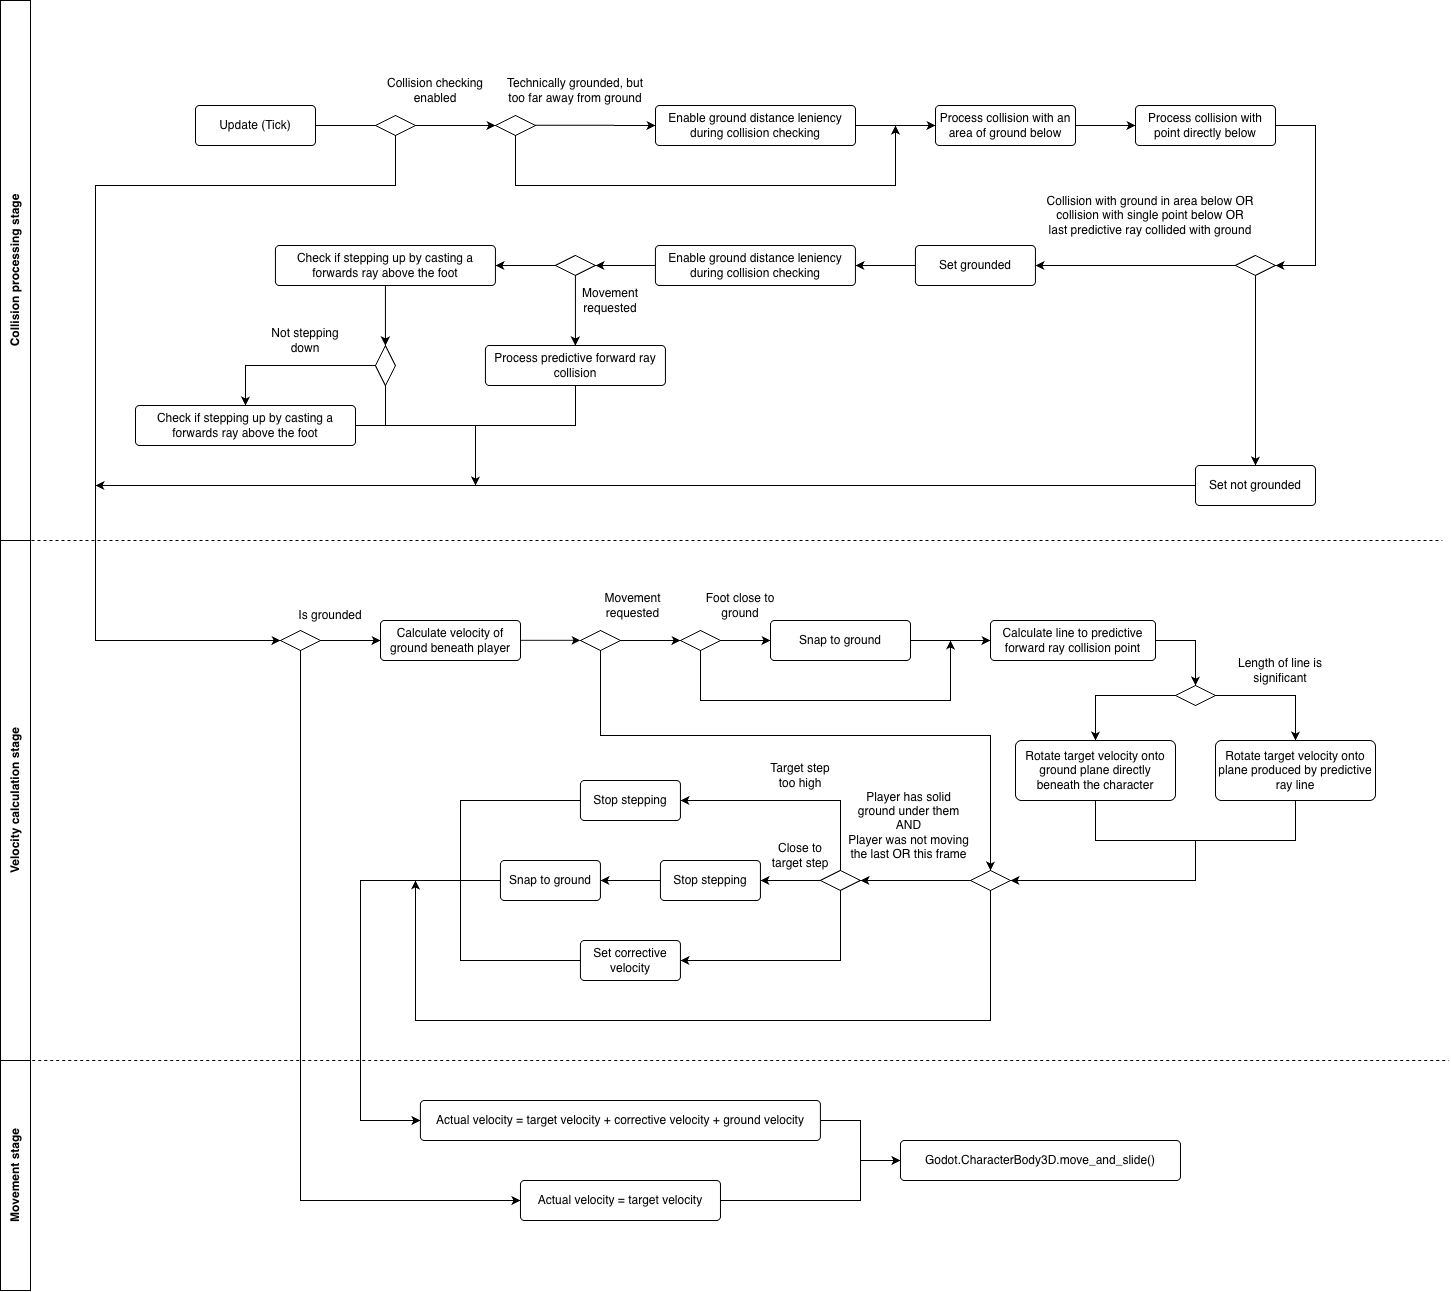
\includegraphics[width=15cm]{../Assets/FloatingBody.png}
    \caption{Aktivitätsdiagramm des FloatingBody-Algorithmus (Eigene Darstellung)}
    \label{fig:floating_body}
\end{figure}

\newpage

\subsubsection{Spieler}

\paragraph{Inheritance-Struktur und Komponentenarchitektur}

Für die Spieler-Architektur wurden die Systeme für den Zustand, die Logik und die physische Darstellung seperariert. Das folgende Klassendiagramm zeigt, wie die Vererbung und Komposition im Detail aufgebaut sind. Basisklassen liefern allgemeine Entity-Eigenschaften wie Animationen, Frame-Daten und Ressourcen, die dann von Entity-Späzifischen Systemen ergänzt werden.

Die \texttt{Player}-Klasse z.B: dient als zentraler Knotenpunkt und bündelt die Sub-Manager für Physik, Input, Kamera und Kampf. Die Bewegung selbst läuft über \texttt{FloatingBody}, das direkt von Godots \texttt{CharacterBody3D} erbt. Dadurch lassen sich die berechneten Bewegungs- und Kollisionsdaten direkt an die Physik-Engine des Frameworks übergeben.


\begin{figure}[h!]
    \centering
    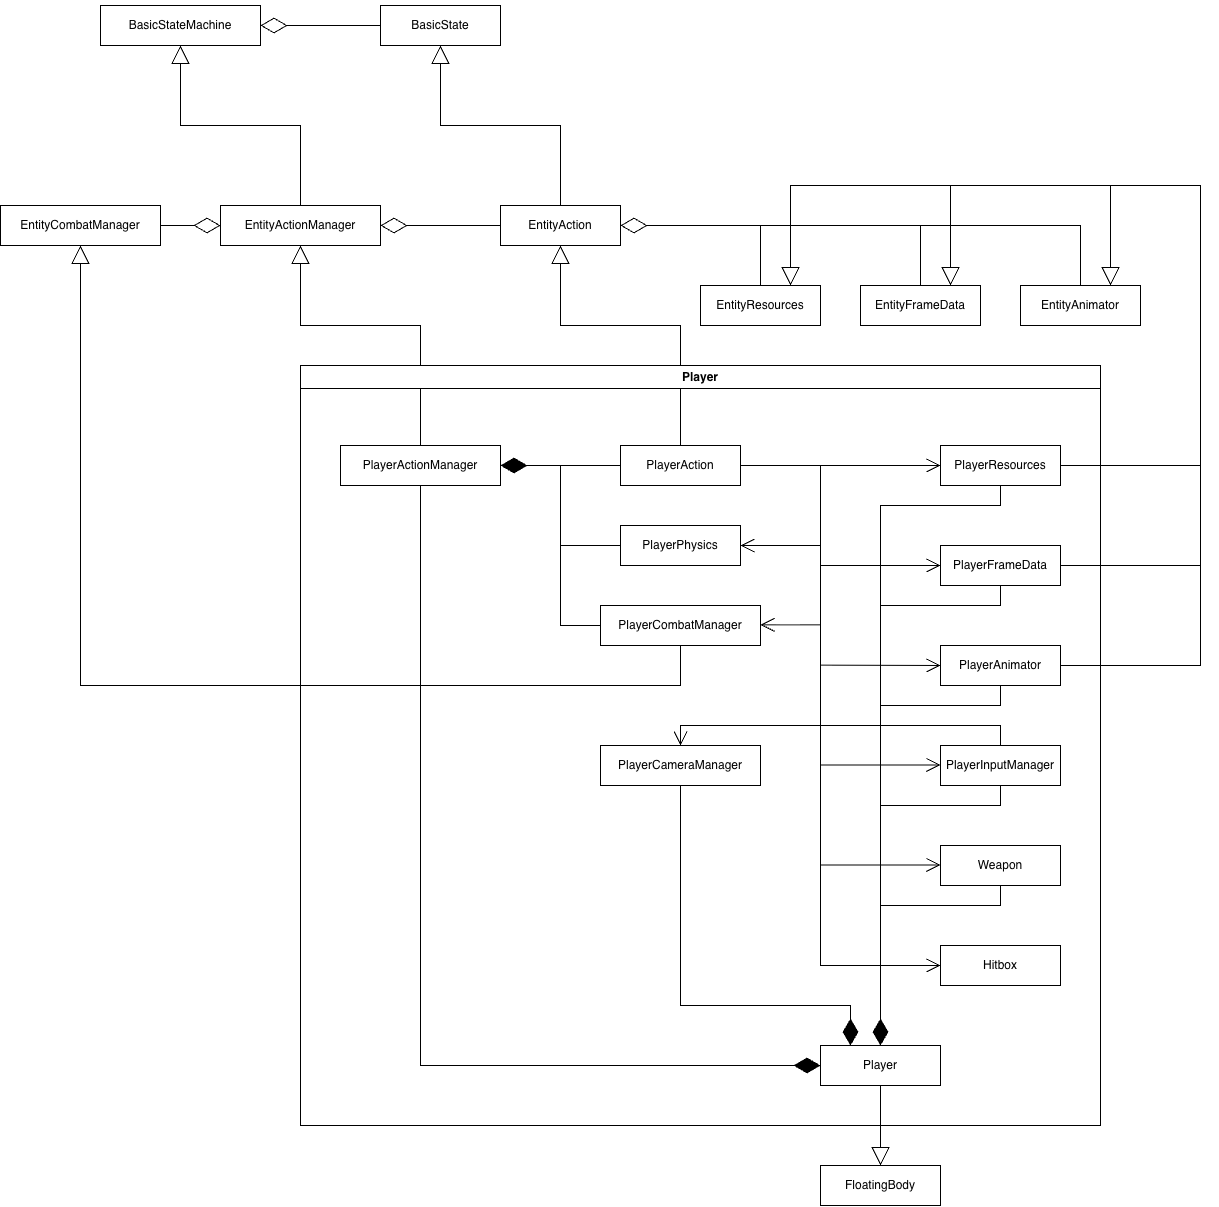
\includegraphics[width=15cm]{../Assets/ClassHierarchy.png}
    \caption{Inheritance-Hierarchie vom Spieler und seinen Komponenten (Eigene Darstellung)}
    \label{fig:class_hierarchy}
\end{figure}

\end{document}